% math4.tex -- sample document (with maths!)
% Fred Barnes, March 2014.

\documentclass[a4paper,12pt]{article}
\usepackage{times}
\usepackage{amsmath}
\usepackage{amsfonts}
\usepackage{graphicx}

\pagestyle{empty}
\renewcommand{\ttdefault}{cmtt}

\begin{document}

\title{How Many Sorts?}
\author{nuked@\#cs}
\date{\today}

\maketitle\thispagestyle{empty}

General question is, how many `{\small\tt sort}' processes are needed to construct an {\bf odd-even sort} (a.k.a.~{\em bricksort}).
The 4-input version looks something like that shown in figure~\ref{fig:sort}:

\begin{figure}[hbt]
	\centering
	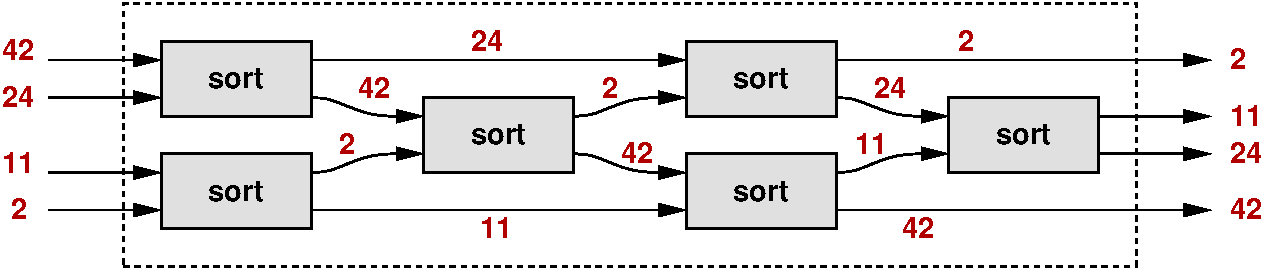
\includegraphics[scale=0.6]{oddevensort.pdf}
	\caption{Odd-even sort, with values.}
	\label{fig:sort}
\end{figure}

For $n$ inputs, there need to be $\frac{n}{2}$ `{\em ranks}', where each rank is a combination of even then odd sort processes.
Within each rank, there are $\frac{n}{2}$ even sorts and $\frac{n}{2} - 1$ odd sorts, giving:
\begin{equation}
	\frac{n}{2} + \biggl(\frac{n}{2} - 1\biggr) = \frac{2n - 2}{2} = n-1
\end{equation}
and then multiplying by the number of ranks required:
\begin{equation}
	\biggl(\frac{n}{2}\biggr) \times (n-1) = \frac{n (n-1)}{2} = \frac{n^2 - n}{2}
\end{equation}
And that's that!

\end{document}
\endinput

